\documentclass[12pt]{article}
\usepackage[utf8]{inputenc}
\usepackage[english]{babel}
\usepackage{amsmath}
\usepackage{amsthm}
\usepackage{graphicx}
\usepackage{epigraph}

\newtheorem{theorem}{}
\newtheorem{exercise}{Exercise}
\newtheorem{problem}{Problem}

\makeatletter
\newenvironment{chapquote}[2][2em]
  {\setlength{\@tempdima}{#1}%
   \def\chapquote@author{#2}%
   \parshape 1 \@tempdima \dimexpr\textwidth-2\@tempdima\relax%
   \itshape}
  {\par\normalfont\hfill--\ \chapquote@author\hspace*{\@tempdima}\par\bigskip}
\makeatother

% CONTENT starts here

\title{\textbf{Exploring Fractals}}
\date{Week 2}
\author{Marko Puza\\}
\begin{document}
\maketitle

\begin{chapquote}{D. Adams, \textit{The Hitchhiker's Guide to the Galaxy}}
\noindent `You know we built planets, do you?' he asked solemnly. \\
`Well yes,' said Arthur, 'I'd sort of gathered...' \\
`Fascinating trade,' said the old man, and a wistful look came into his eyes, `doing the coastlines was always my favourite. Used to have endless fun doing the little bits in fjords...'
\end{chapquote}	

\section{Dimension of fractals}
Roughly speaking, \textbf{fractal} can be described as an object that exhibits a repeating pattern that displays at any scale. Should the replication be same at every scale, it is called a \emph{self-similar}\footnote{intuitevely, the object can be disected into congruent components similar to the original object} pattern. Let's confine our attention on these first.
\\\\
The notion of \textbf{dimension} is usually perceived as number of independent directions, or degrees of freedom, of some object. It turns out that considering the effects of dimension on the measure of similar objects gives a simple way of characterizing fractals. \\
As an ilustration, consider the geometric shapes that we are familiar with first:\\
Suppose we have a line segment of unit length. If we triple the line (expand it by factor of 3), we get a line segment of length three. It contains three congruent components. Note that $3 = 3^1$. \\

\includegraphics{unit_line} \\
Consider a unit square. If we expand the square by the factor of 3, we get a square of area 9 times as great, because it contains 9 copies of the original square. Note that $9 = 3^2$. \\
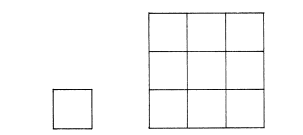
\includegraphics[width = 200px]{square} \\
Finally, consider a unit cube. Again, after expanding the cube by the factor of 3, we get a cube consisting of 27 copies of the original cube. Note here that $27 = 3^3$. \\
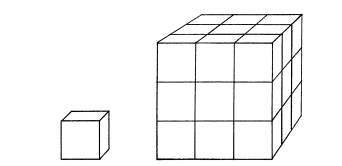
\includegraphics[width = 200px]{cube} \\
Generally, looking at the above	 cases, we have a dimension $d$, a scaling factor $s$ and a number of components (copies) $N$. All of the familiar geometrical shapes seem to fall into the pattern where these three variables are bounded by $N = s^d$.

\begin{exercise}
Can you think of any common geometrical object that is not self-similar? Expand it by the factor of 3. Does $N = s^d$ still hold?  
\end{exercise}

\begin{exercise}
Look at the picture below. Do $N$ and $s$ have to be necessarily integers in order for $N = s^d$ to hold?
\end{exercise}
\centerline{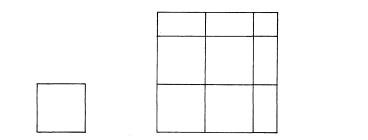
\includegraphics[width = 200px]{non_integer_square}\\}
\noindent What about the dimension\footnote{in the next pages, we will refer by dimension to 'self-similarity' dimension $d$ arising from equation $N = s^d$ (also \textbf{Hausdorff dimension}). Notice that there exist many types of dimensions capturing different concepts.} $d$? One would certainly expect that one to be integer. The Swedish mathematician, Koch, however came up with an geometric construction of an object that, strangely, has non-integral dimension. \\\\
\textbf{Koch snowflake} is constructed as follows: \\
\centerline{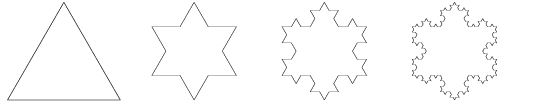
\includegraphics[width = \textwidth]{koch}}\\
Begin with a unit equilateral triangle. Substitute each side of length $l$ (initially 1) by the broken line of length $l\cdot\frac{4}{3}$. (This is just 'popping' a triangle in the middle third of a side) Repeat. The snowflake consist of the region obtained by taking the construction to the limit. 
\begin{exercise}
Find length of the boundary curve of Koch snowflake.
\end{exercise}
\begin{exercise}
Show that area of Koch snowflake is $\frac{2\sqrt{3}}{5}$.
\end{exercise}
\noindent Recall, that area of a unit equilateral triangle is $\frac{\sqrt{3}}{4}$, which means that area of Koch snowflake is $\frac{8}{5}$ the area of the original triangle. \\
While being pretty, we can notice that the snowflake is not self-similar itself. So in order to analyze it's dimension, we need to take a look at a chunk of it that is self-similar. \\
\centerline{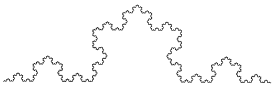
\includegraphics{chunk}} \\
It is possible to disect this chunk into $N = 4$ compontents that are similar to the whole chunk (can you see where to chop?). Each of these components is scaled by scaling factor $s = 3$. Plugging these values into $N = s^d$ finally gives us the dimension of a snowflake $d = \frac{\log{4}}{\log{3}} \approx 1.2619$. \\
The Koch snowflake was one of the first examples of a \emph{fractal} - term devised by B. B. Mandelbrot to describe objects of anomalous dimension.

\begin{exercise}
Consider the \textbf{Menger sponge}\footnote{This is the fractal that decorates the JCMB.}. It is constructed as follows: Begin with a cube. Disect it into 27 equal cubes. Remove the innermost one. Remove the 6 cubes that form centers of faces of the original cube. Repeat on each of the remaining sub-cubes. \\
\centerline{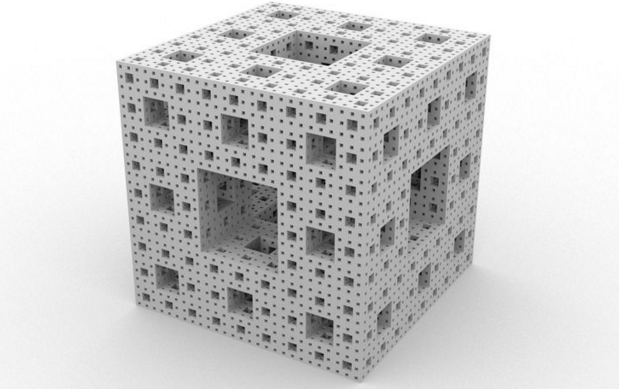
\includegraphics[width = 120px]{sponge}} \\
What is the volume of the Menger sponge? What about its surface area? Is Menger sponge self-similar? Determine the self-similarity dimension of the sponge.
\end{exercise}

\noindent It is not entirely clear what \emph{anomalious} mean in given context - does this include only non-integral dimensions? As it turns out, there exist a fractal which dimension is integral, while it is smaller than we would perhaps expect it to be. 

\begin{exercise}
Lets take look at a three dimensional equivalent of the Sierpiński triangle - the \textbf{Sierpiński tetrahedron}. It can be constructed as follows:
Begin with a regular tetrahedron. Shrink the tetrahedron to half it size and put it's four copies together with corners touching. Repeat the process for each copy.\\
\centerline{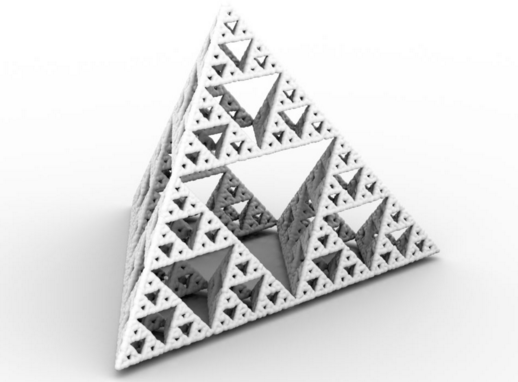
\includegraphics[width = 120px]{tetrahedron}} \\
What is the volume, surface area and self-similarity dimension of the Sierpiński tetrahedron? Notice how the surface area intuitively corresponds to the dimension.
\end{exercise}
\section{L-systems}
\textbf{L-system}\footnote{Lindenmayer system. Originally the L-systems were devised to provide a formal description of the development of fungi and bacteria.} in a fractal context is a tuple of \emph{alphabet} (set of string symbols), \emph{production rules}\footnote{rules that allow expanding symbol into larger string of symbols}, \emph{start string} and some \emph{mechanism to translate generated strings into geometric structure}.\\
While this may sound complicated, the concept is rather simple. The process starts by choosing a start string. Then the production rules are applied iteratively on the string. At each iteration, \textbf{as many as possible} rules are applied (as opposed to formal language, where only one rule per iteration is applied). Generated strings are transformed into geometrical structures. \\
Similarly as classification of formal languages in Chomsky hierarchy\footnote{collection of four classes of formal languages}, we can discern
\textbf{context-free} L-systems (production rules refer only to an individual symbols, not its neighbours, e.g. $A \rightarrow AB$) and \textbf{context-sensitive} L-systems (production rule refers also to a neighbour of a symbol, e.g. $B x \rightarrow B C$). \\
In order to see why L-systems exhibit self-similarity, lets take a look at some famous examples.\\\\
\textbf{Cantor dust}\\
- alphabet: $A,B$\\
- start string: $A$\\
- rules: $A \rightarrow ABA$, $B \rightarrow BBB$\\
- interpretation: A means 'draw forward', B means 'move forward'\\
It can be seen that the first four iterations produce the following strings: \\$A$, $ABA$, $ABABBBABA$, $ABABBBABABBBBBBBBBABABBBABA$\\
Drawing the iterations on the consecutive rows, and considering each row to be of the same length, we end up with the following:\\
\centerline{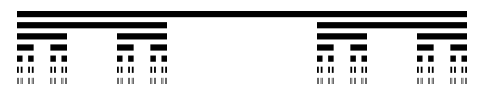
\includegraphics[width = 300px]{dust}}\\
The rows in the above pictures converge towards a \emph{Cantor ternary set} - set of real numbers between zero and one that do not contain digit $1$ in their ternary expansion.
\begin{problem}
Show that the Cantor ternary set $C$ is uncountable\footnote{Find surjective function $f: C \rightarrow [0,1]$}.
\end{problem}
\noindent\textbf{Sierpiński triangle} \\
- alphabet: $A,B,+,-$\\
- start string: $A$\\
- rules: $A \rightarrow +B-A-B+$, $B \rightarrow -A+B+A-$\\
- interpretation: $A,B$ both mean 'draw forward', + means 'turn left by $\frac{\pi}{3}$',\\
\indent\indent\indent\indent\indent$-$ means 'turn right by $\frac{\pi}{3}$'\\
Using turtle graphics with the commands associated with the string gives approximation of the Sierpiński triangle:\\
\centerline{
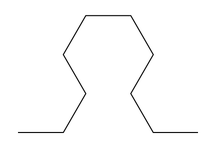
\includegraphics[width = 100px]{sier1}
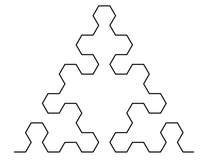
\includegraphics[width = 100px]{sier2}
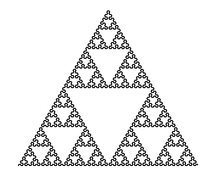
\includegraphics[width = 100px]{sier3}}\\
\begin{exercise}
Consider the following L-system:\\
- alphabet: $A,B$\\
- start string: $A$\\
- rules: $A \rightarrow AB$, $B \rightarrow A$\\
Write down the first few iterations into consecutive rows and draw a line between every alphabet symbol and it's parent. Is the result self-similar? 
\end{exercise}

\section{Fractals in complex plane}
Perhaps the most famous fractals (that are also visualized on a computer most often) are those that are created by iterating maps over the points of complex plane. This gives rise to intricate shapes and colorful images.\\

\noindent \textbf{Mandelbrot set} is defined as a set of all points $c$ on a complex plane such that for given sequence $z_{n+1} = z_{n}^{2} + c$ and starting point $z_0 = 0$  
\[\lim_{n \to \infty} |z_n| \le 2\] \\
In other words, if the above sequence does not diverge for a point of a complex plane, it is part of the set. \\ 
\centerline{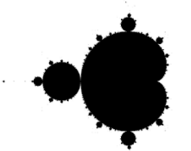
\includegraphics[width = 200px]{mandel}}
Mandelbrot set is often visualized by assigning black color to the points in the set and points outside the set are colored based on how many iterations were completed before $|z_n| > 2$. This is done treating an image as a region of a complex plane, where each pixel represents complex number with corresponding coordinates. Of course, it is only possible to approximate the fractal, thus some threshold $T$ is chosen. If after $T$ iterations we have $|z_T| \le 2$, the point is considered to be part of the set (and thus colored black).
\begin{exercise}
Find the intersection of a Mandelbrot set with real line.
\end{exercise}
\begin{problem}
Show that Mandelbrot set is closed\footnote{For open set S, every point in S has neighbourhood in S. Set is closed if its complement is open.}. \textsc{(hint)}\footnote{\rotatebox{180}{Any intersection of closed sets is closed}}
\end{problem}
\noindent Zooming into various parts of Mandelbrot set gives impression of infinite complexity, which fascinates many people. Similarly as stars in the sky, different parts were named with quite funky names, based on their resemblance. These names include 'double hook', 'seahorse valley', 'elephant valley', 'antenna', 'three headed seahorse' or 'another Mandelbrot'. I recommend taking some time and do some tourism\footnote{$http://guciek.github.io/web\_mandelbrot.html$} in Mandelbrot set.\\
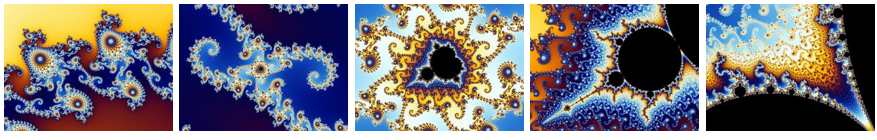
\includegraphics[width = \textwidth]{zoomed_mandel}
Generalization of Mandelbrot sets are Multibrot sets, where the iterations are given by $z_{n+1} = z_{n}^{d} + c$ for some integer $d$.\\

\noindent\textbf{Julia set} has a close relationship to the Mandelbrot set. If $f$ is a function\footnote{entire function} of complex numbers, Julia set of $f$ is the \emph{boundary} of the set of points which diverge under iteration. The \emph{filled Julia set} is a union of Julia set and its interior. \\
Most common Julia sets are defined by quadratic polynomial $f_c(z) = z^2 + c$. Fix a value $c$. The filled Julia set of $f_c$ is set of complex numbers $p$ such that the sequence $z_{n+1} = z_n^2 + c$ does not diverge when starting with $z_0 = p$. \\
Therefore, we obtain different Julia sets for different choices of $c$.\\
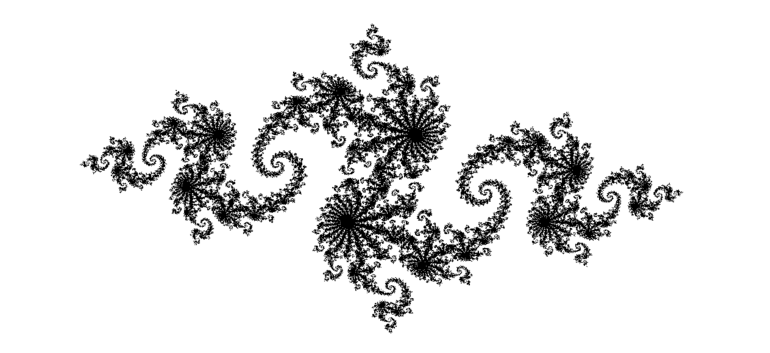
\includegraphics[width = \textwidth]{julia}

\noindent To \textbf{summarize} the difference between Mandelbrot and Julia sets: \\
Consider iteration $z_{n+1} = z_n^2 + c$.\\
$\rightarrow$ Mandelbrot set $M$ records the fate of all possible points $c$ where $z_0 = 0$. \\
$\rightarrow$ Julia set $J_c$ records the fate of all possible starts $z_0$ where $c$ is fixed.\\

\noindent Now we get to the truly interesting part - the theorem that is often regarded as one of the most beautiful results of complex dynamics. \\
\textbf{The fundamental dichotomy} states that either a Julia set is connected or it consists of infinitely many pieces, each of which is a single point\footnote{No matter in what resolution we observe them}. The 'clouds' of these single points are called \emph{Cantor sets} (and often reffered to as 'dusts'). \\
It can be decided whether a Julia set for given $c$ is connected or a Cantor set based on whether the seed $z_0 = 0$ diverges. If it does diverge then the Julia set is a Cantor set, otherwise it is a connected set. To put this in another way:\\ \emph{$J_c$ is connected if $c$ lies in $M$, otherwise it is a Cantor set.}
\begin{exercise}
Realize that this is just a direct consequence of defintion of $M$ and the fundamental dichotomy.
\end{exercise} 
\begin{exercise}
What are the real values of $c$ such that $J_c$ is connected?
\end{exercise} 

\noindent Leaving complex numbers and going two dimensions higher, to the \emph{quaternions} \footnote{Number system that extends the complex numbers - having \emph{1,i,j,k} components}, we can find the Julia sets in the analogical manner. These, being four dimensional, are not that easy to visualize. The only such possibility is to visualize their 3D slices, which are, however, no less mesmerizing.\\
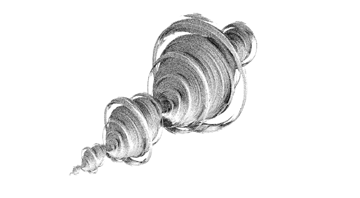
\includegraphics{quatjulia} 


\noindent\textbf{Newton fractal} is a Julia set for the iterations of function $z_{n+1} = z_n - \frac{p(z_n)}{p'(z_n)}$ for a fixed polynomial\footnote{When generating fractal pictures, one can play around and use non-polynomial functions $p$ as well} $p$. Notice that the function above is just a Newton's method for approximating the roots of a polynomial (and thus the name of the fractal). Newton fractal divides a complex plane into regions associated to the roots of the polynomial $p$.\\
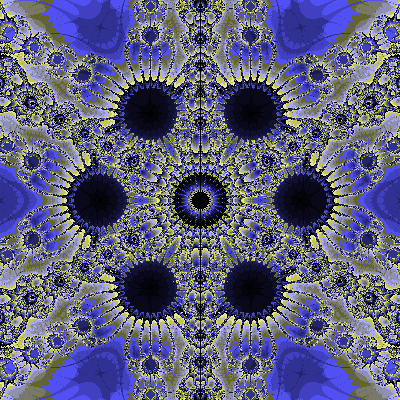
\includegraphics[width = 130px]{example1}
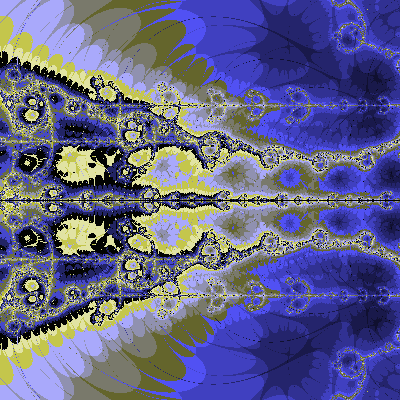
\includegraphics[width = 130px]{example3}
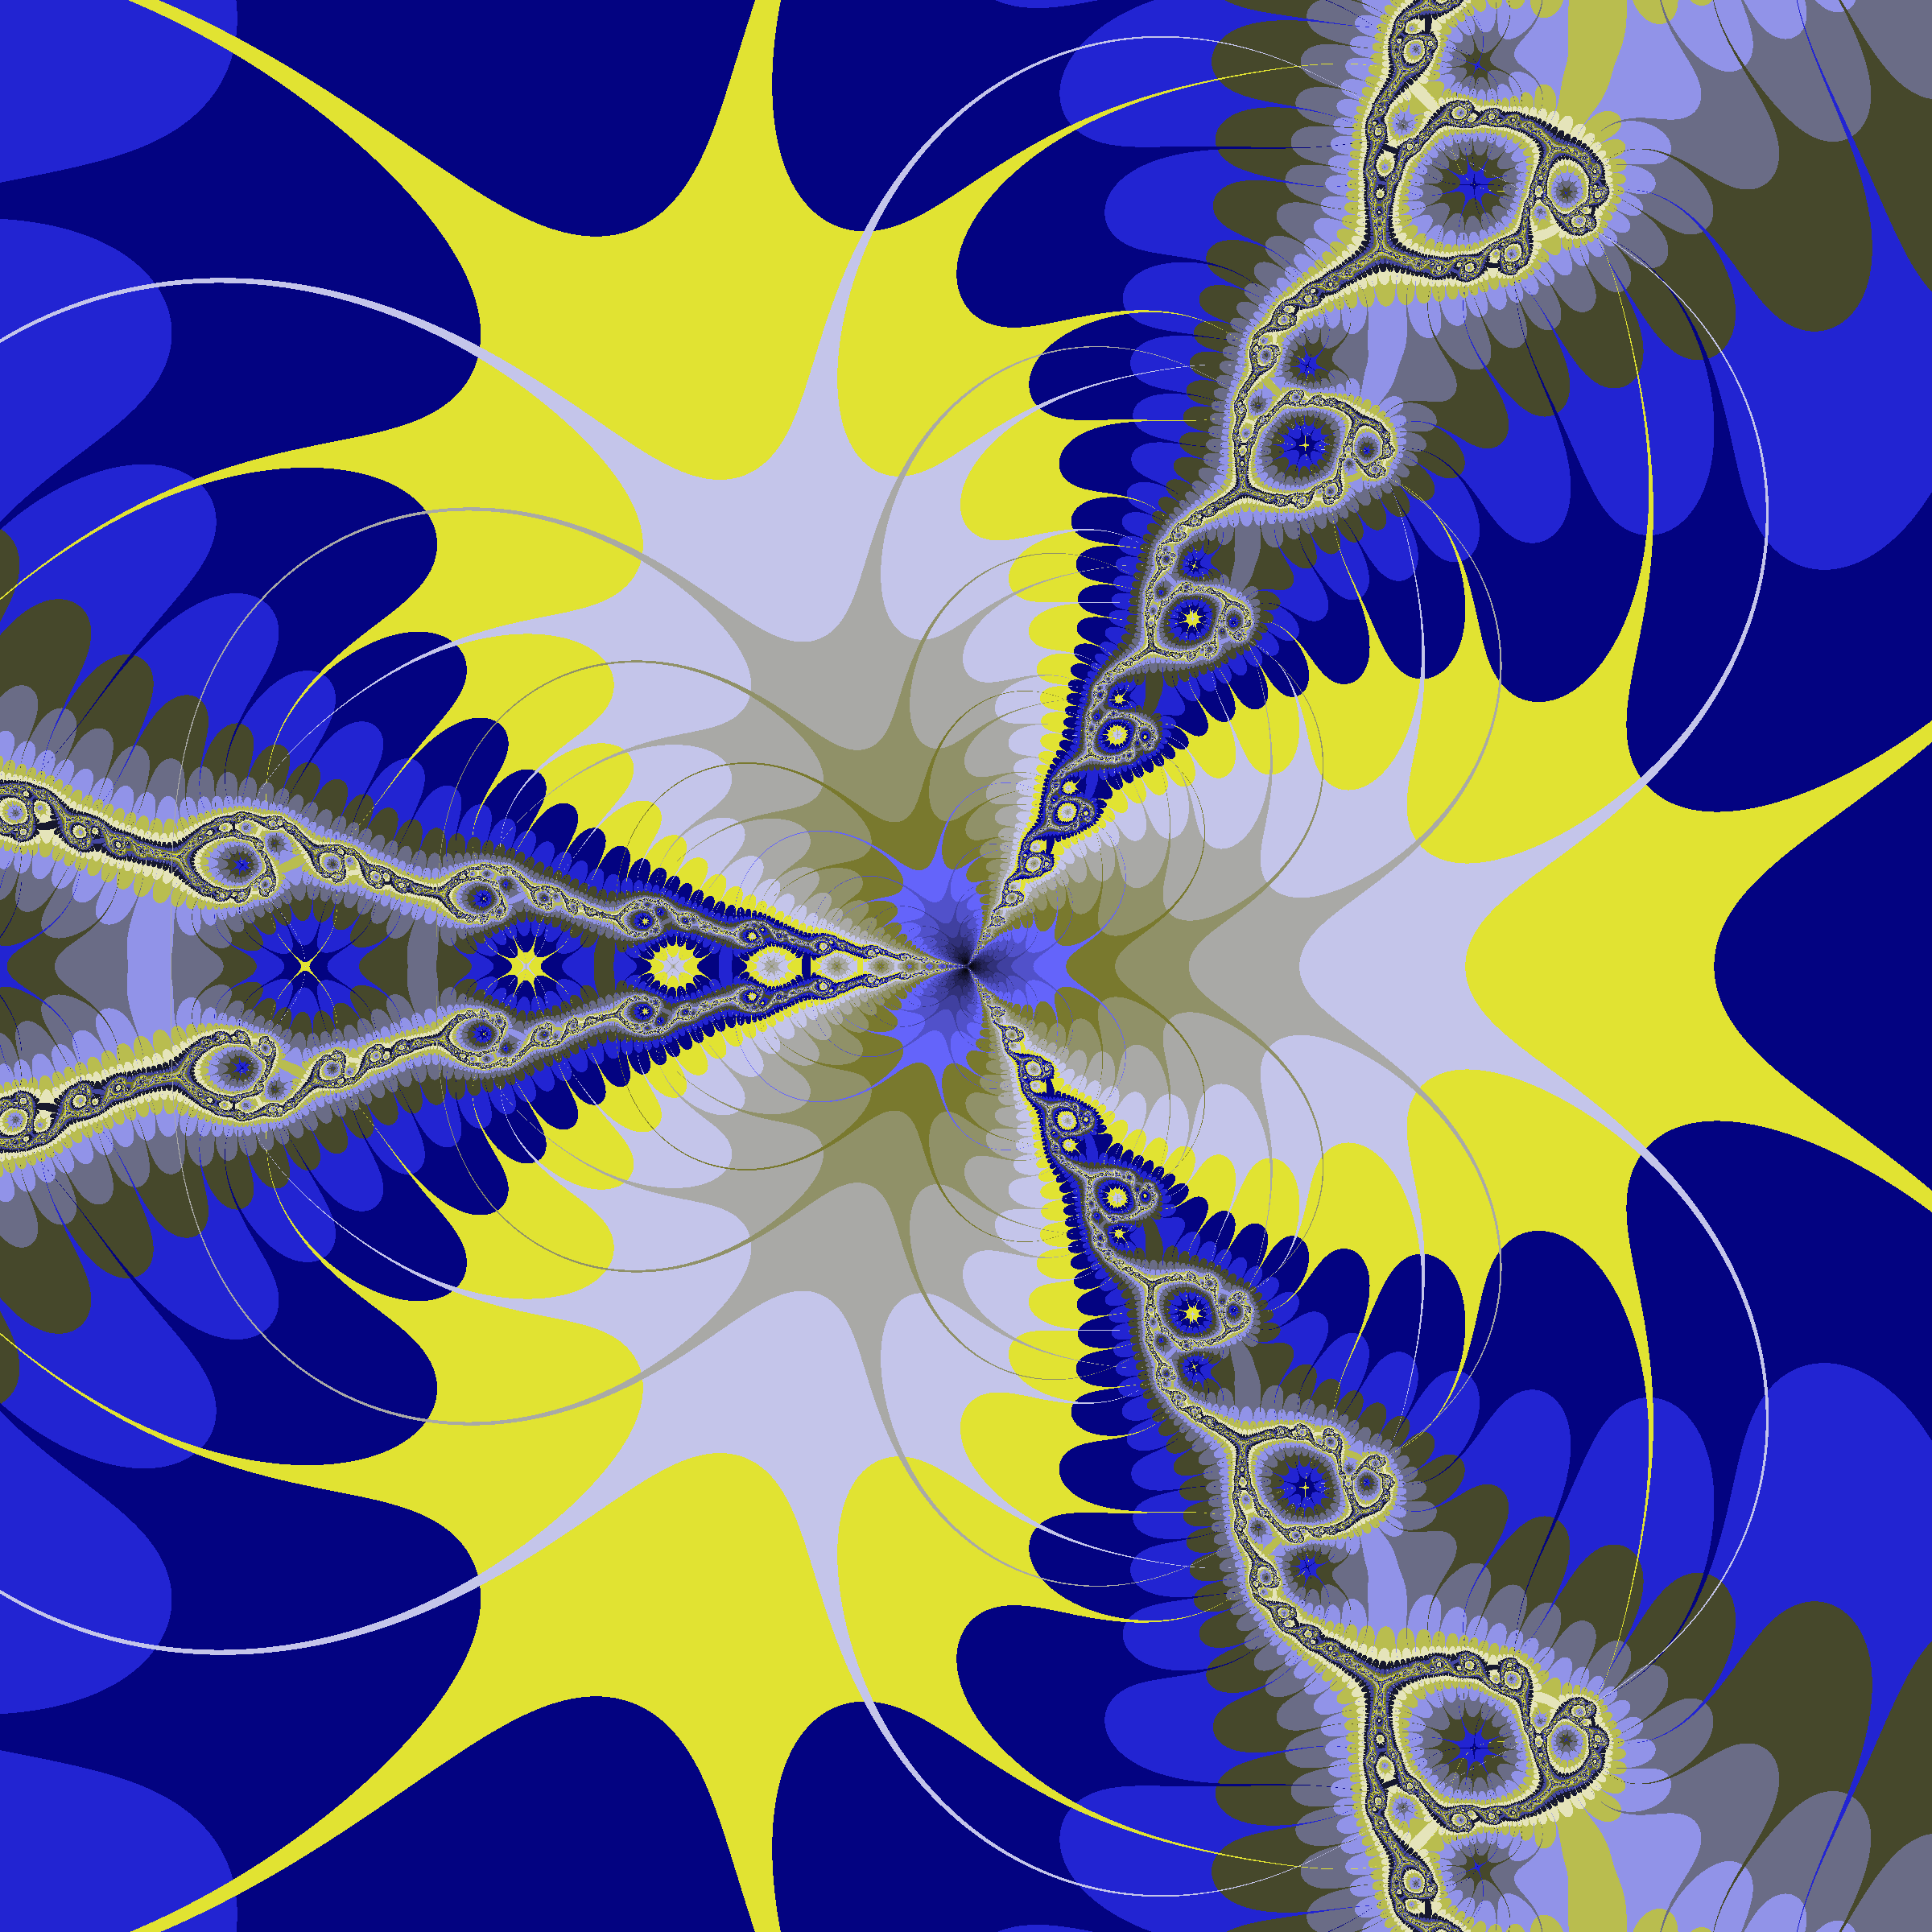
\includegraphics[width = 130px]{example5}

\section{Beyond}

\textbf{Pythagoras tree} Named after the famous Pythagoras theorem, Pythagoras tree can be constructed as follows: take a unit square and construct a right triangle above it's topmost side. The original square's side is a hypotenuse of a triangle - construct squares above it's other sides. Repeat the process for these two new squares, using right triangle with same angles as before.
\centerline{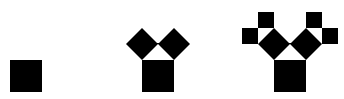
\includegraphics[width = 200px]{tree_constr}}
Taking the repetitions to the limit yields a curious fractal resembling spiral-like tree. Taking a fractal for an isosceles right triangle, it is interesting that the squares start to overlap after $5^{th}$ iteration and the whole tree can actually fit in a $6 \times 4$ rectangle. \\
\centerline{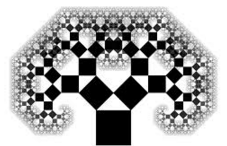
\includegraphics[width = 200px]{tree}}
\begin{exercise}
Show that for the area $A$ of the above Pythagoras tree \[5 < A < 18\].
\end{exercise}

\noindent\textbf{Coastline paradox} is observation the coastline of a landmass behaves fractal-like and does not have a well-defined length. A landmass has features at whatever scale we look at it - ranging from kilometers long coast to tiny specks millimeters long. Therefore, it is not clear what is the smallest feature that should be taken into account when measuring length. This was pointed out by Benoit B. Mandelbrot\footnote{Do you know what B. stands for?}, which resulted in a paper\footnote{`How Long Is the Coast of Britain? Statistical Self-Similarity and Fractional Dimension'}, one of his first about fractals.\\
\centerline{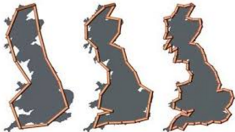
\includegraphics[width = 200px]{coastline}}

\begin{thebibliography}{9}
\bibitem{}Robert L. Devaney. Unveiling the Mandelbrot set. Available at: \texttt{https://plus.maths.org/content/unveiling-mandelbrot-set\\} [Accessed 20 January 2016].

\bibitem{}Paul Bourke. Quaternion Julia Fractals. Available at: \texttt{http://paulbourke.net/fractals/quatjulia/\\} [Accessed 20 January 2016].

\bibitem{}Marko Puza. Newton Flowers. Available at: \\ \texttt{$https://github.com/markopuza/Misc/tree/master/Newton\_Fractals$\\}.

\bibitem{}Anthony Barcellos. The Fractal Geometry of Mandelbrot.

\end{thebibliography}

\end{document}
